\section{An overview of the data}\label{sec:overview}

As was discussed at the end of Section~\ref{subsec:structure}, the majority of
the attributes in the dataset will not be considered at this stage of the
analysis. This allows the focus to be on how the costs of care are distributed
and seen in the data. The subset of chosen attributes will frequently be
referred to as the set of `key attributes' but this choice of name does not
imply that the remaining attributes are not of interest or that they are in any
way unimportant.

The chosen, `key' attributes provide a base for understanding how the
costs and resources consumed by a patient in a spell are built up: cost
components give direct information on which departments and types of procedures
are being utilised; the length of stay can give an indication of the nature of
the spell and any default costs that may be incurred by spending more time in
hospital; and considering the maximum and total number of diagnoses and
procedures (respectively) in a spell allow for some insight into the severity or
complexity of a patient's spell in hospital.


\subsection{Distributions and summative statistics}%
\label{subsec:distributions_statistics}

When looking at the distributions of the key attributes on the whole dataset,
displayed in Figures~\ref{fig:no_spells_bar}~\--~\ref{fig:netcost_kde}, it
is clear that the data is weighted towards low-cost, short-stay, and
otherwise low-impact patients. This behaviour is well-projected through
Figures~\ref{fig:no_spells_bar}~\&~\ref{fig:los_bar}. Here, it is clear that of
all the spells provided under the care of the health board that the majority are
daycases, and that the patients being dealt with are one-time users of the
hospital system.

In general, the distributions themselves have long, pronounced tails. This
suggests that the effect of extreme cases, despite being a rarity, takes a toll
on the hospital system with respect to the cost of providing care.

\begin{figure}[htbp]
    \centering
    \includegraphics[width=\imgwidth]{no_spells_bar/main.pdf}
    \caption{Bar chart for the number of spells associated with a patient.}%
    \label{fig:no_spells_bar}
\end{figure}

\begin{figure}[htbp]
    \includegraphics[width=\imgwidth]{los_bar/main.pdf}
    \caption{Bar chart for the total length of a spell, clipped at 21 days.
        \textit{Maximum 705 days.}}%
    \label{fig:los_bar}
\end{figure}

\begin{figure}[htbp]
    \centering
    \includegraphics[width=\imgwidth]{no_diag_bar/main.pdf}
    \caption{Bar chart for the maximum number of diagnoses in a spell.}%
    \label{fig:no_diag_bar}
\end{figure}

\begin{figure}[htbp]
    \centering
    \includegraphics[width=\imgwidth]{no_proc_bar/main.pdf}
    \caption{Bar chart for the total number of procedures in a spell.}%
    \label{fig:no_proc_bar}
\end{figure}

\begin{figure}[htbp]
    \centering
    \includegraphics[width=\imgwidth]{netcost_kde/main.pdf}
    \caption{Estimated probability density for the net cost of a spell, clipped
        at \pounds12,500. \textit{Maximum approx. \pounds369,000.}}%
    \label{fig:netcost_kde}
\end{figure}

Though the length and returning frequency of the spells are largely minimal and
tightly packed, their associated net costs are wildly variant. This is seen
immediately from inspecting Figure~\ref{fig:netcost_kde}. It would appear that
there is a distinct peak in the figure, but upon closer inspection of the scale
it becomes clear that this peak is little more than a blip; the most probable
net cost has a likelihood of less than one tenth of a percent. The remaining
values are distributed in a way that, given the scale, is near uniform, spanning
from approximately \pounds6000 up to \pounds369,000. A more detailed look at the
skeleton of this distribution, and those of the remaining key attributes, is
given in Table~\ref{tab:summative}.

\begin{table}[htbp]
    \resizebox{\imgwidth}{!}{%
        \begin{tabular}{lrrrrrrrrrr}
\toprule
{} &       COST &       CRIT &      DRUG &      EMER &      ENDO &       HCD &       IMG &   IMG\_OTH &        MED &       NCI \\
\midrule
mean &    1834.93 &     -92.08 &     75.40 &      1.24 &     21.19 &     20.91 &     32.70 &     20.57 &     347.12 &    -30.92 \\
std  &    3771.16 &    1332.61 &    315.17 &     29.13 &     92.76 &    210.98 &    143.67 &    118.26 &     739.73 &     85.80 \\
min  &       4.50 & -250000.61 &     -0.57 &      0.00 &      0.00 &      0.00 &      0.00 &      0.00 &       0.00 & -12960.21 \\
25\%  &     347.67 &       0.00 &      7.18 &      0.00 &      0.00 &      0.00 &      0.00 &      0.00 &      44.45 &    -29.75 \\
50\%  &     749.49 &       0.00 &     20.00 &      0.00 &      0.00 &      0.23 &      0.08 &      0.00 &     130.67 &    -11.64 \\
75\%  &    1886.38 &       0.00 &     59.88 &      0.00 &      0.00 &      4.83 &     10.93 &      0.31 &     375.32 &     -3.02 \\
max  &  369168.93 &       0.00 &  63430.52 &  33347.89 &  11855.95 &  94411.85 &  46708.66 &  46708.66 &  116449.90 &      0.00 \\
\bottomrule
\end{tabular}

    }

    \vspace{5pt}

    \resizebox{\imgwidth}{!}{%
        \begin{tabular}{lrrrrrrrrrr}
\toprule
{} &       NID &    NetCost &     OCLST &       OPTH &      OTH &  OTH\_OTH &      OUTP &        OVH &      PATH &  PATH\_OTH \\
\midrule
mean &     94.83 &    1742.85 &     13.30 &     160.11 &     1.37 &     0.97 &      0.57 &     354.82 &     36.20 &     23.29 \\
std  &    248.16 &    3185.31 &     58.74 &     486.24 &    11.67 &    10.15 &     26.79 &     734.05 &    135.47 &    122.71 \\
min  &      0.00 &       4.50 &      0.00 &       0.00 &     0.00 &     0.00 &      0.00 &       0.00 &      0.00 &      0.00 \\
25\%  &     14.99 &     347.32 &      0.00 &       0.00 &     0.00 &     0.00 &      0.00 &      84.86 &      0.00 &      0.00 \\
50\%  &     32.25 &     747.13 &      0.77 &       0.00 &     0.00 &     0.00 &      0.00 &     139.47 &      4.63 &      0.00 \\
75\%  &     83.36 &    1862.51 &      5.43 &       0.04 &     0.00 &     0.00 &      0.00 &     320.93 &     31.89 &     13.76 \\
max  &  84374.21 &  369168.93 &  12358.37 &  111396.20 &  1248.83 &  1248.83 &  10632.15 &  106428.61 &  70008.12 &  70008.12 \\
\bottomrule
\end{tabular}

    }

    \vspace{5pt}
    
    \resizebox{\imgwidth}{!}{%
        \begin{tabular}{lrrrrrrrrrr}
\toprule
{} &  PATH\_OTH &      PHAR &  PROC\_NO &      PROS &   RADTH &     SECC &       SPS &       THER &  TRUE\_LOS &       WARD \\
\midrule
mean &     23.29 &     30.47 &     1.90 &     40.71 &    0.65 &     0.87 &     11.81 &      28.62 &      2.90 &     497.07 \\
std  &    122.71 &     86.70 &     2.21 &    343.57 &    8.01 &    27.43 &    149.46 &     181.58 &      9.21 &    1236.63 \\
min  &      0.00 &      0.00 &     0.00 &      0.00 &    0.00 &     0.00 &      0.00 &       0.00 &      0.00 &       0.00 \\
25\%  &      0.00 &      2.26 &     0.00 &      0.00 &    0.00 &     0.00 &      0.00 &       0.09 &      0.00 &      10.33 \\
50\%  &      0.00 &      7.24 &     1.00 &      0.00 &    0.00 &     0.00 &      0.00 &       0.63 &      0.00 &     142.01 \\
75\%  &     13.76 &     26.21 &     3.00 &      0.00 &    0.00 &     0.00 &      0.00 &      10.49 &      2.00 &     463.04 \\
max  &  70008.12 &  25087.73 &    70.00 &  33930.70 &  227.64 &  2177.74 &  68029.58 &  125249.49 &   3659.00 &  203854.11 \\
\bottomrule
\end{tabular}

    }
    \caption{Summative spell-level statistics for each of the key attributes.}%
    \label{tab:summative}
\end{table}

Health-related analyses classically categorise patients by grouping ages
together to aid the calculation of risk factors and projected costs. This has
proven to be particularly helpful when looking at older
patients~\cite{Billings327}. Baring this in mind, looking at how age is
distributed amongst the patients in the dataset can provide another valuable
insight into how costs appear.

\begin{figure}[htbp]
    \centering
    \includegraphics[width=\imgwidth]{age_bar/main.pdf}
    \caption{Bar chart for the age of patients in the dataset against the
        estimated UK population in 2016.}%
    \label{fig:age_bar}
\end{figure}

Figure~\ref{fig:age_bar} shows this distribution in contrast to a UK population
estimate in 2016 from the ONS.\@ Following the graph from left to right, the UK
estimate is roughly uniform from birth up until the late 50s where a decline
appears as older people become less prevalent. Looking instead at the patients
in the data it is clear that there are several peaks and troughs. The largest
trough corresponds to adolescents which makes sense since some of the least
likely people to visit a hospital would be reaching their peak fitness
biologically. Similarly, the clear peaks around infancy and in the older age
range correspond to those people who are most vulnerable in terms of their
health. Thus, a hospital should expect to see a disproportionate number of them.


\subsection{Pairwise correlation}\label{subsec:corr}

By looking at the distributions of the key attributes in the previous section,
a surface-level understanding of the data was established. The next logical step
is to dive deeper into the data and investigate how these attributes interact
with one another. In this analysis, correlation coefficients will be used to
give a sense of this interaction.

Figure~\ref{fig:corr_heatmap} shows the Pearson correlation coefficient of all
pairs in the subset of selected attributes. The data has been presented in the
form of a heatmap with a colour bar located to its right, indicating the scale
of the correlation between any two variables. Using a visualisation such as this
is more intuitive than reading directly from the corresponding array of numbers,
and makes gaining insight from the relationships between variables much easier.

The attributes themselves have been arranged into descending order according to
their summed absolute correlation coefficient. Doing this makes it easier to
deduce which variables have the most prominent levels of interaction.

\begin{definition}
    Consider a dataset with \(m \in \mathbb{N}\) attribute columns, denoted
    by \(A = \left\{A_1, \ldots, A_m\right\}\). Attribute \(A_j\) has
    associated with it a summed absolute correlation coefficient, \(c_j\), given
    by:
    
    \[
        c_j = \sum_{k=1}^{m} \left\| \rho_{A_j, A_k} \right\|
    \]

    Here, \(\rho_{A_j, A_k}\) is the Pearson's correlation coefficient
    between attributes \(A_j\) and \(A_k\)
\end{definition}

\begin{figure}[htbp]
    \makebox[\textwidth]{%
        \centering
        \includegraphics[height=.5\paperheight]{corr_heatmap/with_nums.pdf}
    }
    \caption{A heatmap of the pairwise correlation coefficients for the key cost
        attributes. The attributes have been ordered according to their summed
        absolute correlation coefficient.}%
    \label{fig:corr_heatmap}
\end{figure}

Upon inspection of the heatmap, there are many cost components that have no
significant linear correlation with any of the other attributes. Despite this,
however, there are clear correlations between many of the attributes; some of
these are easier to realise than others.

For instance, ignoring the main diagonal, the largest value is that between
total costs (COST) and net costs with a value of 0.94. This indicates almost
total positive linear correlation between these two variables, and that makes
sense given that the net cost of a spell is just the total cost corrected for a
number of reimbursable costs like critical care (CRIT) and non-contracted income
(NCI) which are entered as negative values in the dataset \-- hence their
distinctly negative correlation coefficients with the other variables.
Typically, these deductible costs are small (see Table~\ref{tab:summative}) so a
strong correlation between costs and net costs is to be expected.

Another example is the strong correlation amongst the length of stay
(TRUE\_LOS), and ward and overhead costs (WARD and OVH respectively). These are
well-known relationships that can be justified anecdotally: the longer a patient
spends in hospital, the more time they are likely to spend on a ward. Thus,
incurring associated overheads like administrative work, cleaning costs and a
larger proportion of rental costs. It should also be clear that these attributes
all share a strong linear correlation with the net cost of a spell. This
suggests that these costs and the length of stay are strong indicators of the
net cost of treating someone, and may suggest that the remaining cost components 
make up a substantially smaller part of the net cost.


\subsection{Measuring variation and importance in our cost components}

The larger purpose of this work is to better understand the factors leading to
variations in the cost of treating patients so it would be fitting to
investigate how this variation appears in the cost components. By doing so, a
high level indication of departments and procedures that incur more (or less)
variation can be established. Once a level of variation has been determined, the
relative importance of that component and its variation can be assessed by
considering the overall contribution that component makes to net costs.

In this section, and throughout this analysis, a dimensionless measure of
variation will be used so that the components can be compared against one
another in the same context. This measure is known as the coefficient of
variation and is effectively a normalised standard deviation. During the early
stages of this analysis it was found that the conclusions being made around the
variation in each cost component were flawed since variation was measured using
the classical unbiased sample variance. While this quantity is perfectly valid
and an unbiased estimator for the population variance, it is dependent on the
scale of the data being considered. The effect of this dependency is evident in
Table~\ref{tab:summative}.

\begin{definition}
    Consider a population with mean \(\mu\) and standard deviation \(\sigma\).
    Then the \emph{coefficient of variation}, denoted by \(C_v\), is defined to
    be:

    \[
        C_{v} := \frac{\sigma}{\mu}
    \]

    If only a sample of the data from a population is available then the
    coefficient of variation can be estimated using the sample standard
    deviation and the sample mean analogously.
\end{definition}

In Figure~\ref{fig:cost_variation}, the coefficient of variation for each of the
cost components is shown as a bar chart. The components have been ranked as in
Figure~\ref{fig:corr_heatmap}. It is immediately clear that there are a number
of strongly variant cost components. Take outpatient costs (OUTP) as an example:
its standard deviation is over thirty times the size of its mean. This could go
some way in explaining why there seemed to be no linear correlation with the
other variables in Figure~\ref{fig:corr_heatmap} since these costs are so wildly
varied.

At the other end of the scale, ward and overhead costs have some of the smallest
variations. This would suggest that they are in some way consistent or
predictable, as was commented on in Section~\ref{subsec:corr}. Despite this, the
conclusion is that all of the cost components are still quite highly varied when
considering the entire dataset since the majority of coefficients of variation
found have size far greater than one. 

\begin{figure}[h]
    \centering
    \includegraphics[width=\imgwidth]{cost_variation/main.pdf}
    \caption{Bar chart showing the coefficient of variation \(C_{v}\) of each
        cost component, and the net and total costs.}\label{fig:cost_variation}
\end{figure}

At this point, knowing which of the cost components are the most highly varied
is not sufficient to decide whether they are worth persuing. In order to
determine the relative importance of these findings, the contribution of each
cost component to the net cost of a spell must be considered. Then, with a sense
of the scale of the variation acquired, the components that make the most
significant impacts can be isolated. These quantities are calculated by taking
each cost component in turn, dividing it by its corresponding net cost and
taking the mean over all of these values. This mean is referred as the average
contribution (or proportion) to the net cost, although it is more accurately an
average of the spell-wise ratios between each cost component and the net cost.

\begin{figure}[h]
    \centering
    \includegraphics[width=\imgwidth]{cost_contribution/main.pdf}
    \caption{Bar chart showing the average contribution of each cost component
        to the net cost of a spell.}\label{fig:cost_contribution}
\end{figure}

By inspecting Figure~\ref{fig:cost_contribution}, it is seen that ward, overhead
and medical (MED) costs are the largest contributors to the net cost of a spell
by a large margin. When looking across the remaining bars, the contribution is
substantially smaller for the department-specific cost components. Not only that
but it appears that the most varied components (from
Figure~\ref{fig:cost_variation}) have near negligible average contributions to
the net cost of a spell.

\begin{figure}[h]
    \centering
    \includegraphics[width=\textwidth]{cost_bubble_plot/main.pdf}
    \caption{A bubble plot showing the average contribution to the net cost of a
    spell along the vertical, and the coefficient of variation for that
    component as the size of its marker.}\label{fig:cost_bubble_plot}
\end{figure}

So the question is thus: can these small but highly varied components be
considered especially important? And what about the other components? The
midriffs of each of these figures contain many of the same components but the
relationships are less clear. In order to aid this understanding of how these
two quantities relate to one another, a bubble plot is used. Such a plot allows
three-dimensional data to be displayed in the plane; by running their common
variable along the horizontal axis, both of the quantities can be visualised
together by using the vertical axis and size as two separate dimensions, as
illustrated in Figure~\ref{fig:cost_bubble_plot}.

This figure can be interpreted either by first reading along the vertical axis
to find the components that make the most considerable contribution to treating
a patient, and then investigating the variation that component holds by looking
at the size of its outer marker. The reverse of this process is also perfectly
logical since the objective is to determine where the variation exists, and then
how much of an impact that has on the net cost, as has been done above. The crux
of interpreting this plot is that the further away a large marker is from the
zero line, the more important that component is to be considered. However, small
markers are also of interest since these components indicate that the level of
variation is relatively low \-- the reasons as to why are still unknown.

It is easily seen from this figure that the conclusions made previously still
hold. That is, the largest contributors have some of the smallest measures of
variation while the smallest average contributors are more strongly varied. What
is of interest is the jump between these groups of cost components. There does
not seem to be any particular component in the midriff of contributors that has
large, or indeed small, variation. This suggests that a deeper investigation is
required into individual components and their relationships with specific types
of patient.
